\section{Aufbau der Stoffe}

\subsection{PSE - Periodensystem}

\begin{minipage}[c]{0.4\columnwidth}
	\begin{flushleft}
		\small
		{$\boxed{ \begin{array} {l} Nukleonenzahl \\ = Atommasse = Anzahl_{Protonen} + Anzahl_{Neutronen} \end{array}} \newline
		\boxed{Ladung = Anzahl_{Protonen} - Anzahl_{Elektronen}}$}
	\end{flushleft}

\end{minipage}
\hfill
\begin{minipage}[c]{0.6\columnwidth}
	\tiny{	\begin{flushright}
			\begin{tabular}{l}
				- Protonen und Neutronen sind sog. Nukleonen, \\
				sie wird oftmals auch Massenzahl bezeichnet.  \\
				- Atommasse (Molmasse) [g/mol]
			\end{tabular}
		\end{flushright}
	}
\end{minipage}

\subsection{Stoffe}	
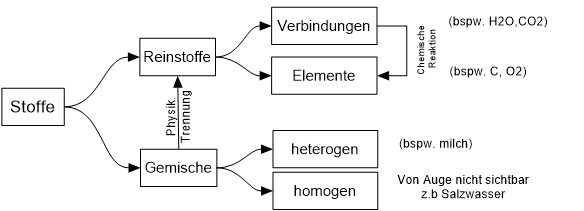
\includegraphics[width=\columnwidth]{images/Stoffe_RM.png}
\renewcommand{\arraystretch}{1.0}

\subsection{Aggregatzustand}		

{\footnotesize
	\begin{tabular}[\columnwidth]{l l | l l}
		\underline{\textbf{Aggregatzustand}} &                              & \underline{\textbf{Dispersitätsgrad}} &                          \\
		\textbf{Dispersionsmittel}           & \textbf{Dispergierter Stoff} & \textbf{Heterogen}                    & \textbf{Homogen}         \\
		gasförmig (g)                        & gasförmig (g)                & -                                     & Gasgemisch               \\
		gasförmig (g)                        & flüssig (l)                  & Nebel                                 & -                        \\
		gasförmig (g)                        & fest (s)                     & Rauch                                 & -                        \\
		flüssig (l)                          & gasförmig (g)                & wenig haltbarer Schaum                & Gaslösung                \\
		flüssig (l)                          & flüssig (l)                  & wenig haltbare Emulsion               & Flüssigkeitslösung       \\
		flüssig (l)                          & fest (s)                     & Suspension                            & feststofflösung          \\
		fest (s)                             & gasförmig (g)                & fester Schaum*                        &                          \\
		fest (s)                             & flüssig (l)                  & brei                                  &                          \\
		fest (s)                             & fest (s)                     & Feststoffgemische                     & legierung zweier Metalle \\
		*( zB. Schaumstoff)                  &                              &                                       &
	\end{tabular} 
}
		
\subsection{Eselsbrücke}
\small{
\begin{tabular}{ll} 
	\textbf{HONClBrIF – "der Brief vom Onkel"}   &  Die Buchstaben stellen dabei \\
	& die Elemente des PSE dar, die in der \\
	& Natur nur 2-atomig vorkommen. \\ 
	\hline
	Ausnahme: & $P_4$ (Phosphor) und $S_8$ (Schwefel)  \\
\end{tabular}
}

\subsection{Isotope}
\small{\begin{tabular}{l}
	\textbf{Isotope} sind Nuklide (=gleichen Atomsorte) mit der gleichen Ordnungszahl    \\
	(=Protonen),
	\textbf{aber unterscheiden sich von der Anzahl Neutronen}.             \\
	Die meisten \underline{natürlichen Elemente haben ein oder paar stabile Isotope,}    \\
	während andere Isotope vom gleichen Element \underline{radioaktiv} sind (=instabil). \\
	Dann spricht man von $\alpha , \beta , \gamma -Zerfall$ .
\end{tabular}
}

\subsection{Kugelwolkenmodell}	
\begin{center}
	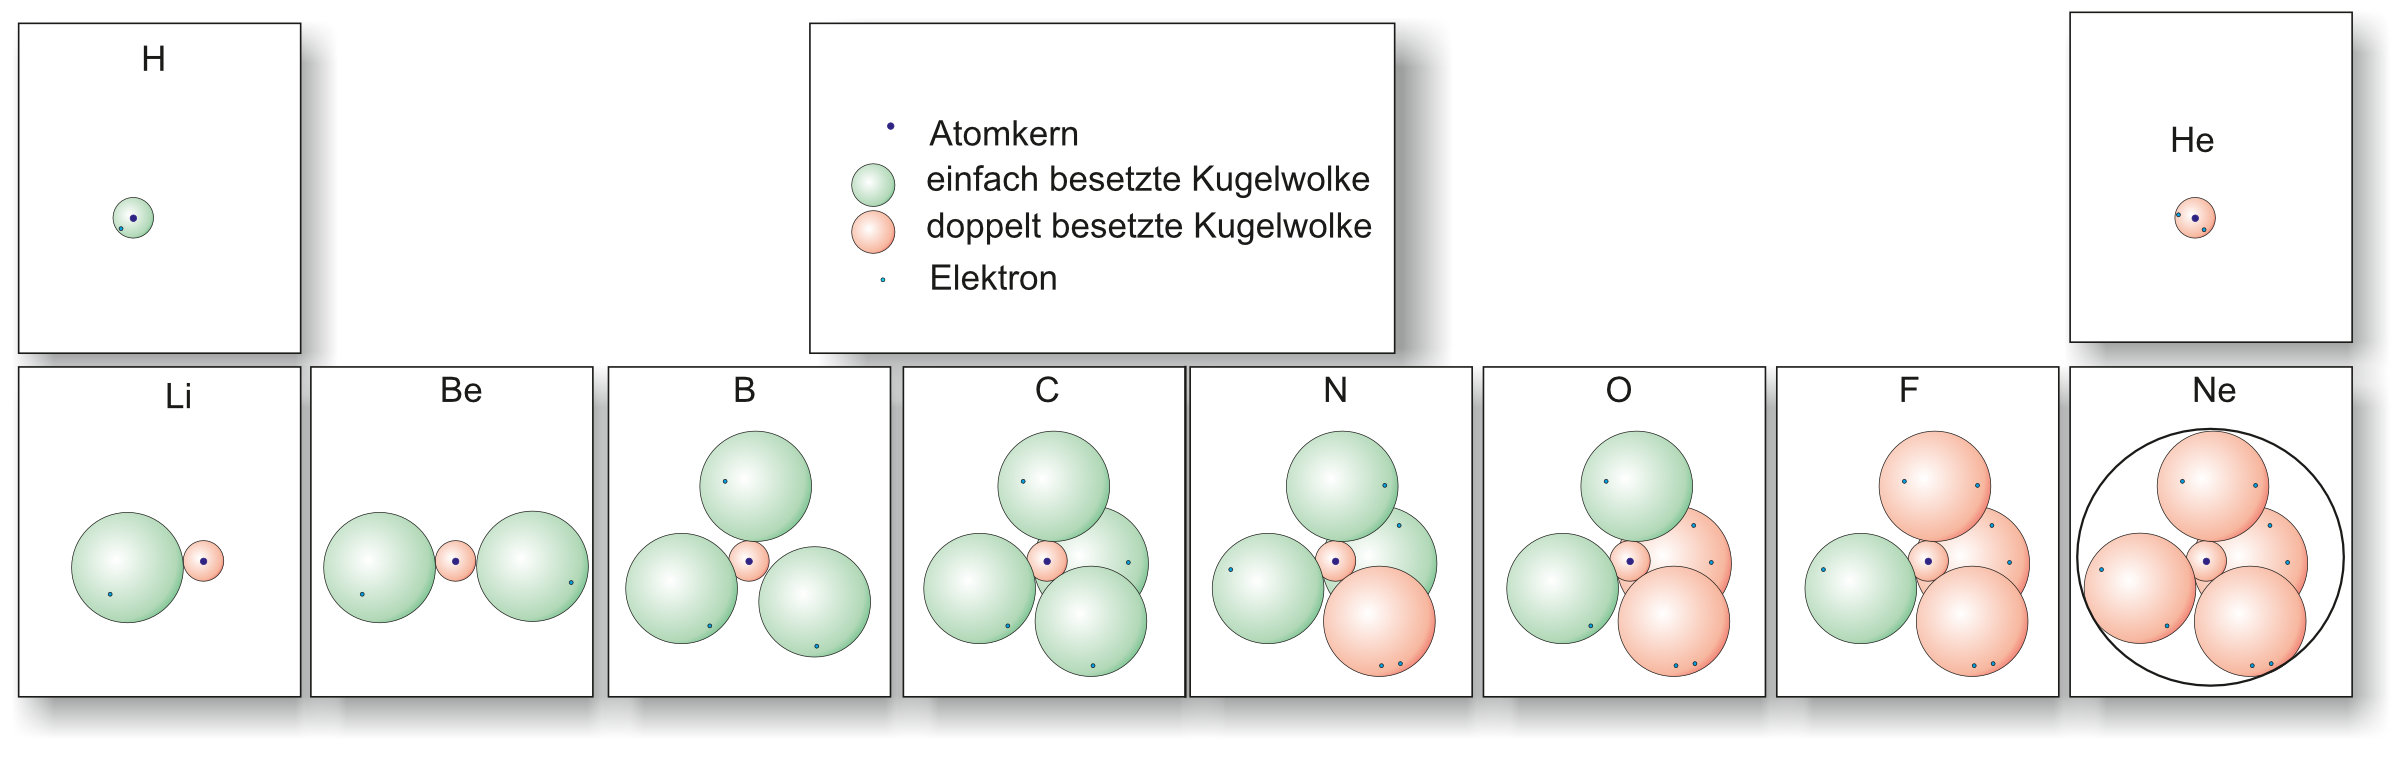
\includegraphics[width=\columnwidth]{images/kugelwolkenmodell.jpg}
\end{center}

\subsection{Schreibweisen von Lewis} 

\begin{center}
	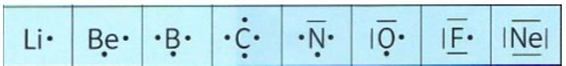
\includegraphics[width=\columnwidth]{images/Lewis-schreibweise_2.png}
\end{center}

\begin{flushleft}
	\includegraphics[width=0.7\columnwidth]{images/lewis-schreibweise.png}
\end{flushleft}
\small{
\begin{tabular}{ll}
	\textbf{VE Hauptgruppen (1-8)}~ &  im PSE bestimmbar \\
	\textbf{VE Nebengruppen}  &  komplizierter/unmöglich, nicht Prüfungsrelevant\\
	\hline
	\textbf{Beispiel}: & Natrium (Na): 1. Hauptgruppe = 1 Ve \\
	& Kohlenstoff (C): 4. Hauptgruppe = 4 Ve  \\
\end{tabular}
}
